\section{Fizyka}\label{sec:fizyka}

Ważnym elementem gry jest fizyka, aby postaci mogły poruszać się, podskakiwać i reagować na kolizje.

Podstawowym komponentem zapewniającym obliczenia fizyczne jest \name{Rigidbody}. Komponent ten przyjmuje parametry takie jak wartość masy, tarcia, czy wyłączenie grawitacji.

Aby zdarzenia fizyczne mogły mieć miejsce, na elementy otoczenia oraz samą postać gracza nałożone powinny zostać komponenty \name{Collider}. Są to obszary określające granice kolizji. Mogą one mieć kształt kapsuły, sześcianu, bądź uproczczonego modelu samego obiektu. Pozwalają one silnikowi gry na przyspieszenie obliczeń i płynne reakcje na zdarzenia kolizji.

\begin{figure}[H]
\center
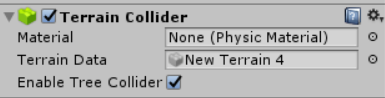
\includegraphics[width=6cm]{fizyka_1.png}
\caption{Przykład -- collider mapy terenu}
\end{figure}

W przypadku postaci poruszających się po mapie, zablokowane zostały obroty we wszystkich osiach (parametr \name{Freeze Rotation} komponentu Rigidbody), dzięki czemu nie przewracają się one na bok przy nierównościach terenu i kolizjach z otoczeniem. Zdarzenia fizyczne wyliczane są jedynie w pionie (spadanie, skok itp.).

\subsection{Mechanika skakania postaci}

Mając już zaimplementowaną fizykę, dodaliśmy możliwość skoku. Utworzona została metoda \textit{jump()}, która dodaje do zdarzeń fizycznych naszej postaci siłę w kierunku pionowym o wektorze ustalonym parametrem \textit{jumpPower}. Natomiast na podstawie kolizji z terenem ustalane jest, czy postać stoi na ziemi, dzięki czemu nie można wykonać kolejnego skoku będąc już w powietrzu.
\\
\begin{lstlisting}[caption={Fragment algorytmu skoku postaci}]
void Start()
{
    rb = GetComponent<Rigidbody>();
    anim = GetComponent<Animator>();
}

void jump()
{
    if (onGround)
    {
        onGround = false;
        rb.AddRelativeForce(new Vector3(0, jumpPower, 0));
        anim.SetTrigger("Jump");
    }
}

void OnTriggerEnter(Collider other)
{
    onGround = true;
}
\end{lstlisting}